\documentclass[10pt]{beamer}
\usepackage[utf8]{inputenc}
\usepackage[T1]{fontenc} 
\usepackage[croatian]{babel}
\usepackage{fix-cm}
\usetheme[progressbar=frametitle]{metropolis}
\usepackage{appendixnumberbeamer}
\usepackage{booktabs}
\usepackage{pgfplots}
\usepgfplotslibrary{dateplot}
\usepackage{xspace}
\graphicspath{ {slike/} }
\newcommand{\themename}{\textbf{\textsc{metropolis}}\xspace}
\usepackage{times}

\title{Git submoduli}
\subtitle{mogućnost korištenja repozitorija unutar repozitorija}
\date{}
\author{Dario Barać, Anđelo Ferenčić}

\begin{document}
\nocite{*}
\maketitle

%\begin{frame}{Table of contents}
% \setbeamertemplate{section in toc}[sections numbered]
%  \tableofcontents[hideallsubsections]
%\end{frame}


\begin{frame}{Uvod u git submodule}
\begin{itemize}
	\item Ako razvijamo projekt unutar kojeg se nalazi drugi projekt (npr. Bootstrap library unutar repozitorija web sjedišta) može doći do problema sa praćenjem njihovih verzija.
	\item Git taj problem riješava sa submodulima koji nam omogućuju njihovo neovisno verzioniranje.
\end{itemize}	
\end{frame}

\begin{frame}[fragile]{Početak rada sa submodulima}
 	U repozitoriju našeg web sjedišta ćemo inicijalizirati git submodul za Bootstrap library koristeći naredbu: \begin{semiverbatim}$submodule add \end{semiverbatim}
 	Submodul će biti spremljen u poddirektorij projekta i imat će isti naziv kao originalni repozitorij kojeg uključujemo.

	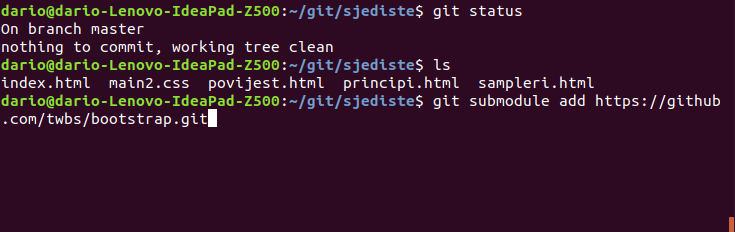
\includegraphics[scale=0.35]{submoduli_pocetak}
\end{frame}

\begin{frame}[fragile]{Početak rada sa submodulima}
	Naredba \begin{semiverbatim}$git status \end{semiverbatim} nam javlja daje stvorena .submodule datoteka koja sadrži imena i url adrese svih submodula. 

	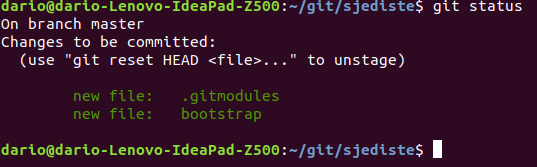
\includegraphics[scale=0.45]{submoduli_status}

	Možemo primjetiti i da git ne prati \emph{bootstrap}-ove datoteke jer zna da je to podrepozitorij.
\end{frame}

\begin{frame}{Početak rada sa submodulima}
	I kada napravimo \emph{commit} git prati podrepozitorije kao samo jednu datoteku.

	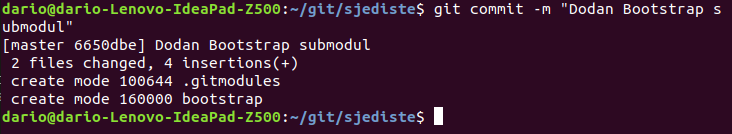
\includegraphics[scale=0.42]{sub_commit}

\end{frame}

\begin{frame}[fragile]{Kloniranje submodulima}
	Kada kloniramo repozitorij dobijemo dobijemo i prazan direktorij njegovih submodula. \\
	Sljedeće naredbe dohvaćaju sve datoteke koje su potrebne za rad podrepozitorija:
	\begin{semiverbatim}$git submodule init \end{semiverbatim}
	\begin{semiverbatim}$git submodule update \end{semiverbatim}
\end{frame}

\begin{frame}[fragile]{Kloniranje submodulima}
	Brža alternativa za to je da kod kloniranja dodamo i:
	\begin{semiverbatim} --recurse-submodules\end{semiverbatim}

	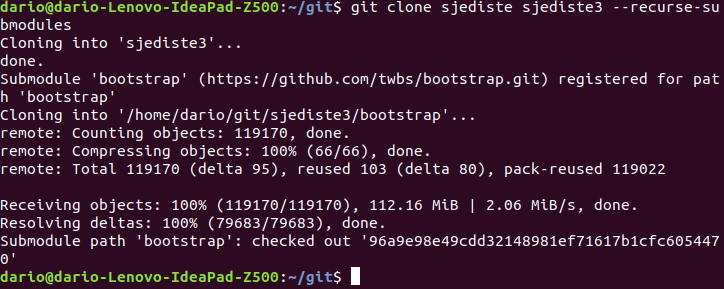
\includegraphics[scale=0.42]{sub_recurse}
\end{frame}

\begin{frame}[fragile]{Rad na projektima sa submodulima}
	Sadržaj podrepozitorija u našem projektu možemo ažurirati tako da unutar njihovih direktorija napišemo ove naredbe:
	\begin{semiverbatim}$git fetch\end{semiverbatim}
	\begin{semiverbatim}$git merge\end{semiverbatim}
	Ako imamo više podrepozitorija u projektu, ažuriranje nam može oduzeti dosta vremena.
\end{frame}

\begin{frame}[fragile]{Rad na projektima sa submodulima}
	To se rješava u glavnom direktoriju projekta sljedećom naredbom:
	\begin{semiverbatim}$git submodule update ---remote\end{semiverbatim}
	Time smo ažurirali sve submodule u našem projektu.

	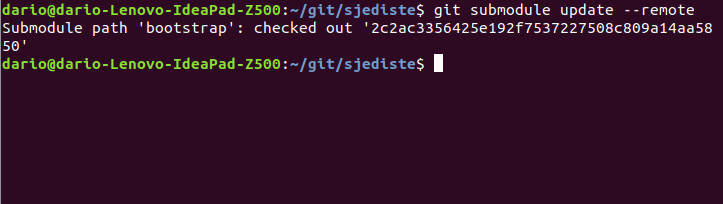
\includegraphics[scale=0.4]{sub_update}
\end{frame}

\begin{frame}[fragile]{Rad na projektima sa submodulima}
	\begin{semiverbatim}$git status\end{semiverbatim}
	U glavnom direktoriju javlja da imamo nove \emph{commitove} u podrepozitorijima.

	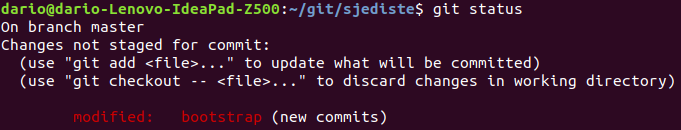
\includegraphics[scale=0.4]{sub_status2}

	\begin{semiverbatim}$git diff ---submodule\end{semiverbatim}
	Pokazuje koji su to \emph{commitovi}:

	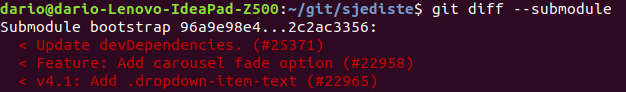
\includegraphics[scale=0.4]{sub_diff2}
\end{frame}

\begin{frame}[fragile]{Rad na submodulima}
    Koristeći naredbu  
    \begin{semiverbatim}$git submodule update \end{semiverbatim}   
    Git pribavlja promjene i ažurira datoteke u poddirektoriju, no nijedna grana ne prati naše promjene u podrepozitoriju.
    
\end{frame}

\begin{frame}[fragile]{Rad na submodulima}
    
    Da bismo riješili taj problem moramo napraviti dvije stvari:
    \begin{itemize}
    \item Ući u svaki submodul i "\emph{checkout}"-at granu na kojoj ćemo raditi.
    \item Konfigurirati što će Git napraviti ako smo napravili promjenu te onda naredbom
     \begin{semiverbatim}$git submodule update ---remote \end{semiverbatim}
    pullamo nove promjene.
    \end{itemize}
\end{frame}

\begin{frame}[fragile]{Rad na submodulima}
    
    Dodavanjem \begin{semiverbatim}---merge\end{semiverbatim} na korišteni git update poziv spojit ćemo promjenu koja je na serveru za ovaj submodul sa našom granom.
    \begin{semiverbatim}$git submodule update ---remote ---merge \end{semiverbatim}

    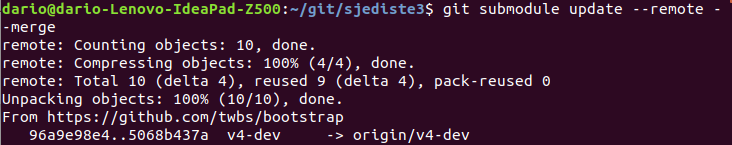
\includegraphics[scale=0.4]{sub_merge}
\end{frame}

\begin{frame}[fragile]{Rad na submodulima}
    Dodavanjem
    \begin{semiverbatim}---rebase\end{semiverbatim}
    spojit ćemo promjenu našu lokalnu promjenu sa serverom.
\end{frame}

\begin{frame}[fragile]{Objavljivanje promjena na submodulima}
    
    Ako imamo promjene na glavnom projektu i lokalne promjene u submodulu i commitamo glavni projekt i pushamo ga bez pushanja promjena na submodulu ostali koji rade na projektu neće imat pristup promjenama na submodulu. 
    
\end{frame}


\begin{frame}[fragile]{Objavljivanje promjena na submodulima}
    
    Da bismo ovaj problem riješili na naredbu
    \begin{semiverbatim}git push\end{semiverbatim}
    nadodamo argument \begin{semiverbatim}---recurse-submodules\end{semiverbatim}
    koji može biti "check" ili "on-demand".
    
    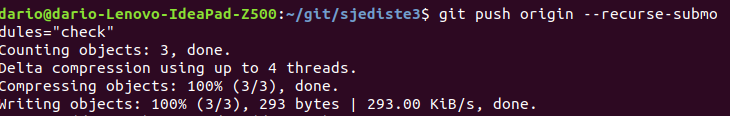
\includegraphics[scale=0.4]{sub_check}
\end{frame}

\begin{frame}[fragile]{Objavljivanje promjena na submodulima}
    
    "check" opcija samo javi da promjene na submodulu nisu pushane te zaustavi push.
    "on-demand" opcija pokuša pushati promjene na submodulima i nakon toga glavni projekt.

    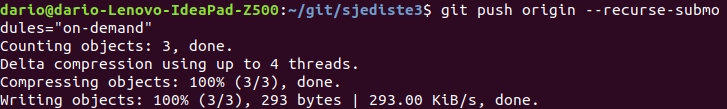
\includegraphics[scale=0.4]{sub_ondemand}
    
\end{frame}

\begin{frame}[fragile]{Foreach naredba}
    
    Ako imamo više submodula u istom projektu naredba foreach olakšava stvari.
	Npr. ako izradimo novu granu i želimo se prebaciti na nju na svim submodulima.
	
    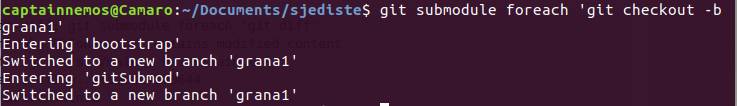
\includegraphics[scale=0.4]{sub_foreach}
\end{frame}

\begin{frame}[fragile]{Problemi sa submodulima}
    
    Grananje sa submodulima može biti problematično.
    Ako napravimo novu granu, dodamo submodul na tu granu i vratimo se na granu bez tog submodula još uvijek imamo direktorij submodula kao nepraćeni direktorij.
    
    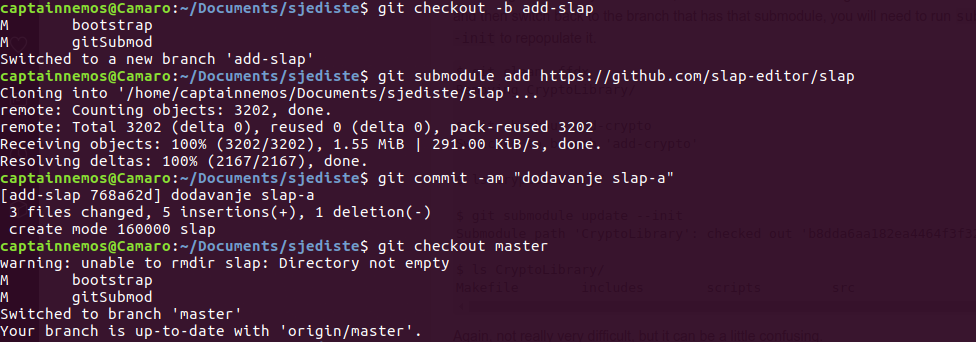
\includegraphics[scale=0.3]{sub_removing_sub1}
\end{frame}

\begin{frame}[fragile]{Problemi sa submodulima}
    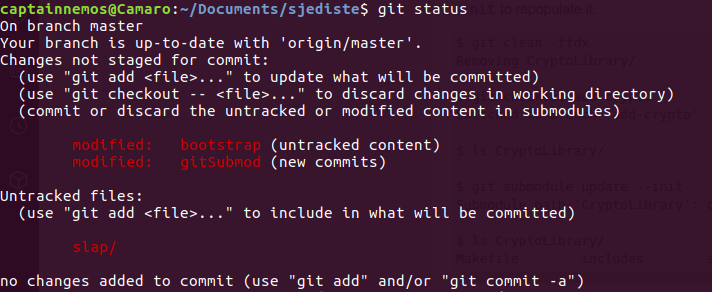
\includegraphics[scale=0.34]{sub_removing_sub2}
    
    Ako izbrišemo taj direktorij, nakon što se ponovo vratimo na granu sa submodulom moramo pozvati naredbu
    \begin{semiverbatim}git submodule update --init\end{semiverbatim}
    da bi ponovo je popunili.

\end{frame}

\begin{frame}[fragile]{Problemi sa submodulima}
    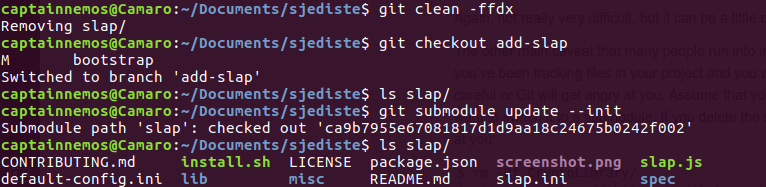
\includegraphics[scale=0.4]{sub_removing_sub3}
    
    Mijenjanje iz poddirektorija u submodule je također jedan od čestih problema.
    Mora se unstageat poddiretorij i tek onda se može dodati submodul.
    
\end{frame}

\begin{frame}[fragile]{Literatura}
	\bibliographystyle{ieeetr}
  	\bibliography{Pro_Git}
\end{frame}
\end{document}